
%(BEGIN_QUESTION)
% Copyright 2006, Tony R. Kuphaldt, released under the Creative Commons Attribution License (v 1.0)
% This means you may do almost anything with this work of mine, so long as you give me proper credit

Anta at et trykkmåler bruker en membran som trykksensor, slik:

$$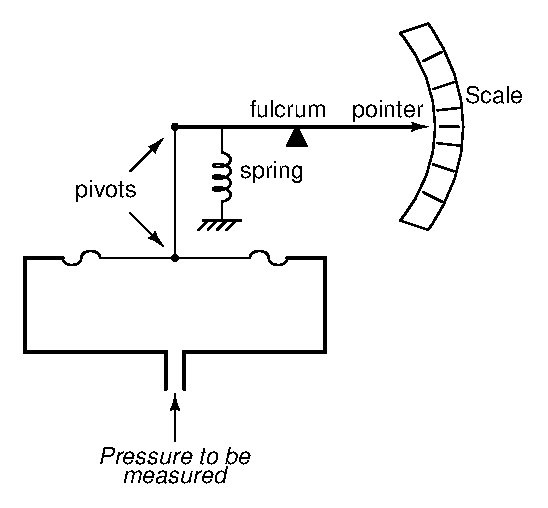
\includegraphics[width=15.5cm]{i00172x01.eps}$$

Denne mekanismen virker, men hva hvis vi ønsker å gjøre den mer følsom?  Det vil si: vi ønsker mindre måleområde slik at lavere trykk gir fullt utslag på viseren.  Hva kan endres i mekanismen for å redusere måleområdet?

\underbar{file i00172}
%(END_QUESTION)





%(BEGIN_ANSWER)

Mulige endringer for å gjøre denne trykkmålemekanismen mer følsom:

\begin{itemize}
\item{} Øk membranarealet
\item{} Reduser fjærkonstanten i membranen
\item{} Flytt vippepunktet mot linken, til venstre, bort fra skalaen
\end{itemize}

%(END_ANSWER)





%(BEGIN_NOTES)


%INDEX% Measurement, pressure: diaphragm

%(END_NOTES)
